\documentclass[10pt,a4paper]{article}
\usepackage[a4paper,margin=24mm]{geometry}
\usepackage{newtxtext,newtxmath}
\usepackage{graphicx}
\usepackage{booktabs}
\usepackage{array}
\usepackage{amsmath}
\usepackage{amssymb}
\usepackage{float}
\usepackage{caption}
\usepackage{setspace}
\usepackage{titlesec}
\usepackage{fancyhdr}
\usepackage{enumitem}
\usepackage[hidelinks]{hyperref}

\setlength{\parindent}{0pt}
\setlength{\parskip}{4pt}
\linespread{1.0}
\pagestyle{fancy}
\fancyhf{}
\fancyfoot[C]{\thepage}
\renewcommand{\headrulewidth}{0pt}

\titleformat{\section}{\fontsize{11}{13}\bfseries}{\thesection.}{0.6em}{}
\titleformat{\subsection}{\fontsize{10}{12}\bfseries}{\thesubsection}{0.6em}{}
\captionsetup{font=small}

\begin{document}

% Official conference header provided by organizer
\begin{center}
    
\includegraphics[width=\textwidth]{eesconf.ir_1758539471.png}
\end{center}

\vspace{2mm}

{\centering\fontsize{12}{14}\bfseries
EHPRA: Enhanced Hybrid Probabilistic Routing Algorithm with Smart Detour for\
Fault- and Congestion-Aware 2D Mesh NoC\par}

\vspace{6mm}

{\centering\fontsize{10}{12}\bfseries Amir Ahkbari\par}
{\centering\fontsize{10}{12}\itshape MSc. student of Amirkabir University of Technology\par}

\vspace{2mm}

{\centering\fontsize{10}{12}\bfseries Hosein Khoojooyan\par}
{\centering\fontsize{10}{12}\itshape MSc. student of Amirkabir University of Technology\par}

\vspace{2mm}

{\centering\fontsize{10}{12}\bfseries Dr. Mohsen Tarighi\par}
{\centering\fontsize{10}{12}\itshape Professor at Amirkabir University of Technology\par}

\vspace{6mm}

{\fontsize{11}{13}\bfseries Abstract}\par
Network-on-Chip (NoC) routing in many-core systems must satisfy two conflicting requirements: low-latency packet delivery and resilience against congestion-induced failures in heavily used links. This paper presents EHPRA (Enhanced Hybrid Probabilistic Routing Algorithm), a lightweight extension of HPRA for 2D mesh NoCs that introduces a Smart Detour mechanism to improve routing quality under hotlink and hotspot traffic conditions. Unlike random detour approaches, EHPRA evaluates multiple intermediate candidates and selects the least congested path using a destination-aware congestion score plus a hop penalty. The algorithm preserves HPRA's probabilistic adaptation concept while improving path selection quality through local link-usage history. A simulation framework on a 16$\times$16 mesh compares EHPRA against HPRA, Minimal-Oblivious, Random Detour, and XY routing over one million trials per scenario. Results show that EHPRA achieves the lowest fault counts in both hotspot (150,320) and hotlink (213,375) tests. Compared with HPRA, EHPRA reduces faults by 10.29\% in hotspot traffic and 27.20\% in hotlink traffic. Although EHPRA may increase average hops versus strictly minimal algorithms, it provides the best reliability-latency trade-off, achieving the minimum weighted overall cost across all compared methods.

\textbf{Keywords:} Network-on-Chip, 2D Mesh, Adaptive Routing, Fault Tolerance, Congestion Awareness, Smart Detour, HPRA, EHPRA

\section{Introduction}
Network-on-Chip (NoC) has become the default interconnect paradigm for many-core processors because shared-bus structures no longer scale with core count, memory pressure, and mixed traffic classes. In a regular 2D mesh topology, deterministic routing is easy to implement and verify, but heavy communication concentration in practical workloads can create repeated contention on specific links. Under such stress, packets repeatedly traverse the same channels, and any temporary or persistent disturbance can significantly degrade throughput, latency, and fairness.

The challenge is stronger when traffic is non-uniform. Two traffic patterns are particularly important for evaluating adaptive routing under stress: \emph{hotlink} and \emph{hotspot}. In hotlink traffic, one source-destination corridor dominates communication and repeatedly activates the same short path region. In hotspot traffic, many sources target one destination region, creating destination-centric convergence and increased pressure on links near the sink. In both cases, minimal-path preference alone is insufficient for robust operation because it does not actively avoid overloaded or repeatedly faulty links.

Hybrid Probabilistic Routing Algorithm (HPRA) was proposed to improve robustness by combining minimal and detour routes under an adaptive probability variable $p$. HPRA established a useful framework where the router can switch exploration intensity according to observed faults. However, classical HPRA still leaves a key gap: once detour is selected, intermediate-node selection is not fully congestion-informed and can still produce avoidable path costs.

This paper proposes EHPRA, an enhanced variant that preserves HPRA's adaptive framework while replacing random detour behavior with a \emph{Smart Detour} mechanism. Smart Detour evaluates multiple candidate intermediates, scores complete paths using historical link usage and destination-aware weighting, and chooses the lowest-cost detour candidate. This design keeps state and arithmetic lightweight while systematically improving detour quality.

The contributions of this paper are:
\begin{enumerate}[leftmargin=6mm]
    \item A destination-aware Smart Detour strategy integrated into a probabilistic hybrid routing framework.
    \item A practical scoring function that couples congestion history with bounded hop penalty.
    \item A reproducible, large-scale comparison against HPRA, Minimal-Oblivious, Random Detour, and XY routing in a 16$\times$16 mesh.
    \item Expanded analysis on reliability-latency trade-off, complexity, implementation feasibility, and parameter sensitivity.
\end{enumerate}

\section{Background and Related Routing Approaches}
\subsection{Deterministic Dimension-Ordered Routing (XY)}
XY routing resolves horizontal displacement first and vertical displacement second. It is deadlock-free for mesh and has minimal hardware overhead. Nevertheless, deterministic behavior leads to severe path concentration under non-uniform traffic and makes heavily used links recurring points of failure.

\subsection{Minimal-Oblivious Routing}
Minimal-oblivious routing introduces random intermediate coordinates while preserving minimality from source to intermediate and intermediate to destination. It improves path diversity compared with strict XY but does not directly use congestion state. Therefore, link-history awareness remains limited.

\subsection{Random Detour Routing}
Detour routing routes packets outside the source-destination bounding box to bypass crowded regions. Uninformed detours can reduce repeated local pressure, but they may increase path length dramatically and remain unpredictable in quality.

\subsection{Hybrid Probabilistic Routing Algorithm (HPRA)}
HPRA combines minimal-oblivious and detour behavior through adaptive probability $p$. After a fault event in minimal mode, $p$ increases (more exploration); after a fault event in detour mode, $p$ decreases (less exploration). A decay term gradually returns $p$ toward low values. HPRA is effective but still sensitive to detour quality.

\subsection{Research Gap}
Existing approaches either (i) stay too rigid (XY), (ii) diversify but remain congestion-unaware (minimal-oblivious), or (iii) detour without informed candidate ranking (random detour and basic HPRA detour). EHPRA addresses this gap with explicit candidate scoring and destination-centric congestion weighting.

\section{System Model and Problem Formulation}
\subsection{Topology and Routing Domain}
We consider a 2D mesh NoC of size $R\times C$ with bidirectional links between adjacent routers. Each router is represented by coordinates $(r,c)$ and unique node identifier. A packet routing decision must produce a legal path $P = [n_0, n_1, \dots, n_k]$ from source $n_0$ to destination $n_k$.

\subsection{Traffic and Fault Assumptions}
Two traffic regimes are studied:
\begin{itemize}[leftmargin=6mm]
    \item \textbf{Hotlink}: fixed source and destination repeatedly communicating.
    \item \textbf{Hotspot}: random source nodes communicating with a single destination.
\end{itemize}
Faults are modeled as temporarily faulty links selected from high-usage candidates. During fault duration, any path that traverses the active faulty link incurs a fault event.

\subsection{Optimization Objective}
The routing objective is multi-criteria: minimize fault exposure while preserving reasonable path length. A weighted metric is used for aggregate comparison:
\begin{equation}
\mathrm{Cost} = w_f \cdot \frac{F}{F_{\max}} + w_h \cdot \frac{H}{H_{\max}},\quad w_f=0.8,\;w_h=0.2
\end{equation}
where $F$ is total faults and $H$ is average hops. Lower cost implies a better reliability-latency compromise.

\section{Proposed EHPRA Method}
\subsection{Hybrid Decision Core}
EHPRA keeps HPRA's mode-selection logic. For every packet, two route candidates are available:
\begin{enumerate}[leftmargin=6mm]
    \item Minimal-oblivious route.
    \item Smart-detour route.
\end{enumerate}
A random draw $r\sim U(0,1)$ chooses detour when $r<p$; otherwise minimal-oblivious is used.

\subsection{Adaptive Probability Update}
The adaptation law is event-driven:
\begin{itemize}[leftmargin=6mm]
    \item If fault occurs under minimal mode: $p \leftarrow \min(1, p + p_{up})$.
    \item If fault occurs under detour mode: $p \leftarrow \max(0, p - p_{down})$.
    \item Every trial: $p \leftarrow \max(0, p - p_{decay})$.
\end{itemize}
This provides gradual exploration-exploitation balancing.

\subsection{Smart Detour Candidate Generation}
Let source and destination define a bounding box. EHPRA samples up to $k$ candidate intermediate nodes and encourages off-box exploration with detour radius:
\begin{equation}
\Delta = \max\left(1, \left\lfloor p\cdot\max(R,C)\cdot k_{\Delta}\right\rfloor\right)
\end{equation}
Higher $p$ allows farther candidates, increasing bypass flexibility during persistent congestion.

\subsection{Destination-Aware Scoring}
For each intermediate candidate, EHPRA builds complete path $P$ and evaluates
\begin{equation}
\mathrm{Score}(P)=\sum_{(u,v)\in P} w(u,v)\cdot U(u,v)+\lambda\cdot H(P)
\end{equation}
where $U(u,v)$ is link usage history and $H(P)$ is hop count. The destination-aware weight is
\begin{equation}
w(u,v)=1+\frac{6}{d+1}
\end{equation}
with $d$ the Manhattan distance from link endpoints to destination. Hence, congestion near destination is penalized more.

\subsection{Algorithmic Workflow}
The EHPRA routing loop can be summarized as follows:
\begin{enumerate}[leftmargin=6mm]
    \item Build minimal-oblivious path and Smart-Detour candidate paths.
    \item Score candidate detours and choose minimum-score detour path.
    \item Select minimal or detour mode using probability $p$.
    \item Update link usage counters from selected path.
    \item Apply fault check and update $p$ according to mode/fault condition.
\end{enumerate}
This workflow uses only local counters and simple arithmetic operations.

\subsection{Complexity Discussion}
Assuming $k$ detour candidates and average path length $\bar{L}$, per-packet detour evaluation costs approximately $\mathcal{O}(k\bar{L})$ in the simulator. Because $k$ is bounded (default 12) and path generation relies on deterministic primitives, the method remains computationally practical for software simulation and potential hardware-inspired approximation.

\begin{figure}[H]
    \centering
    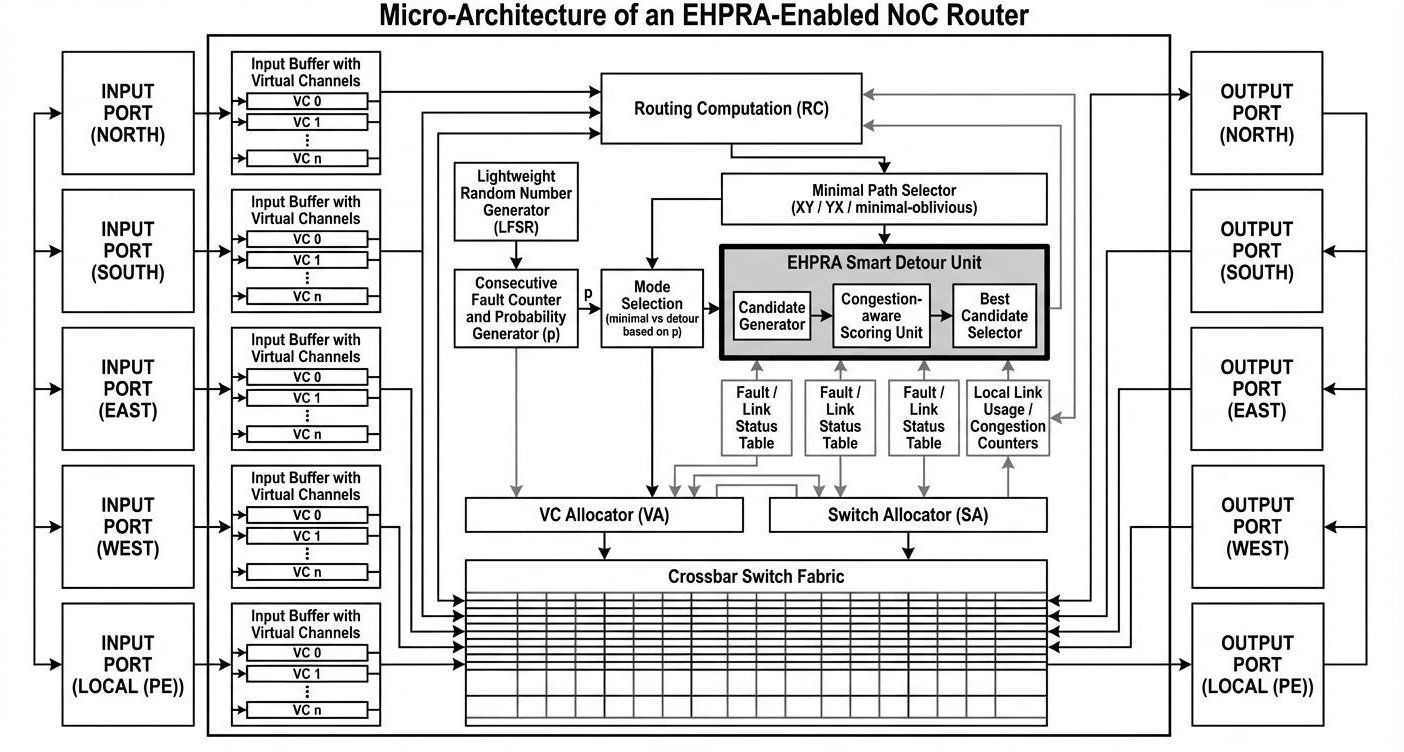
\includegraphics[width=0.68\textwidth]{Results/RouterArchitecture.jpeg}
    \caption{Routing architecture used in the simulator workflow.}
\end{figure}

\begin{figure}[H]
    \centering
    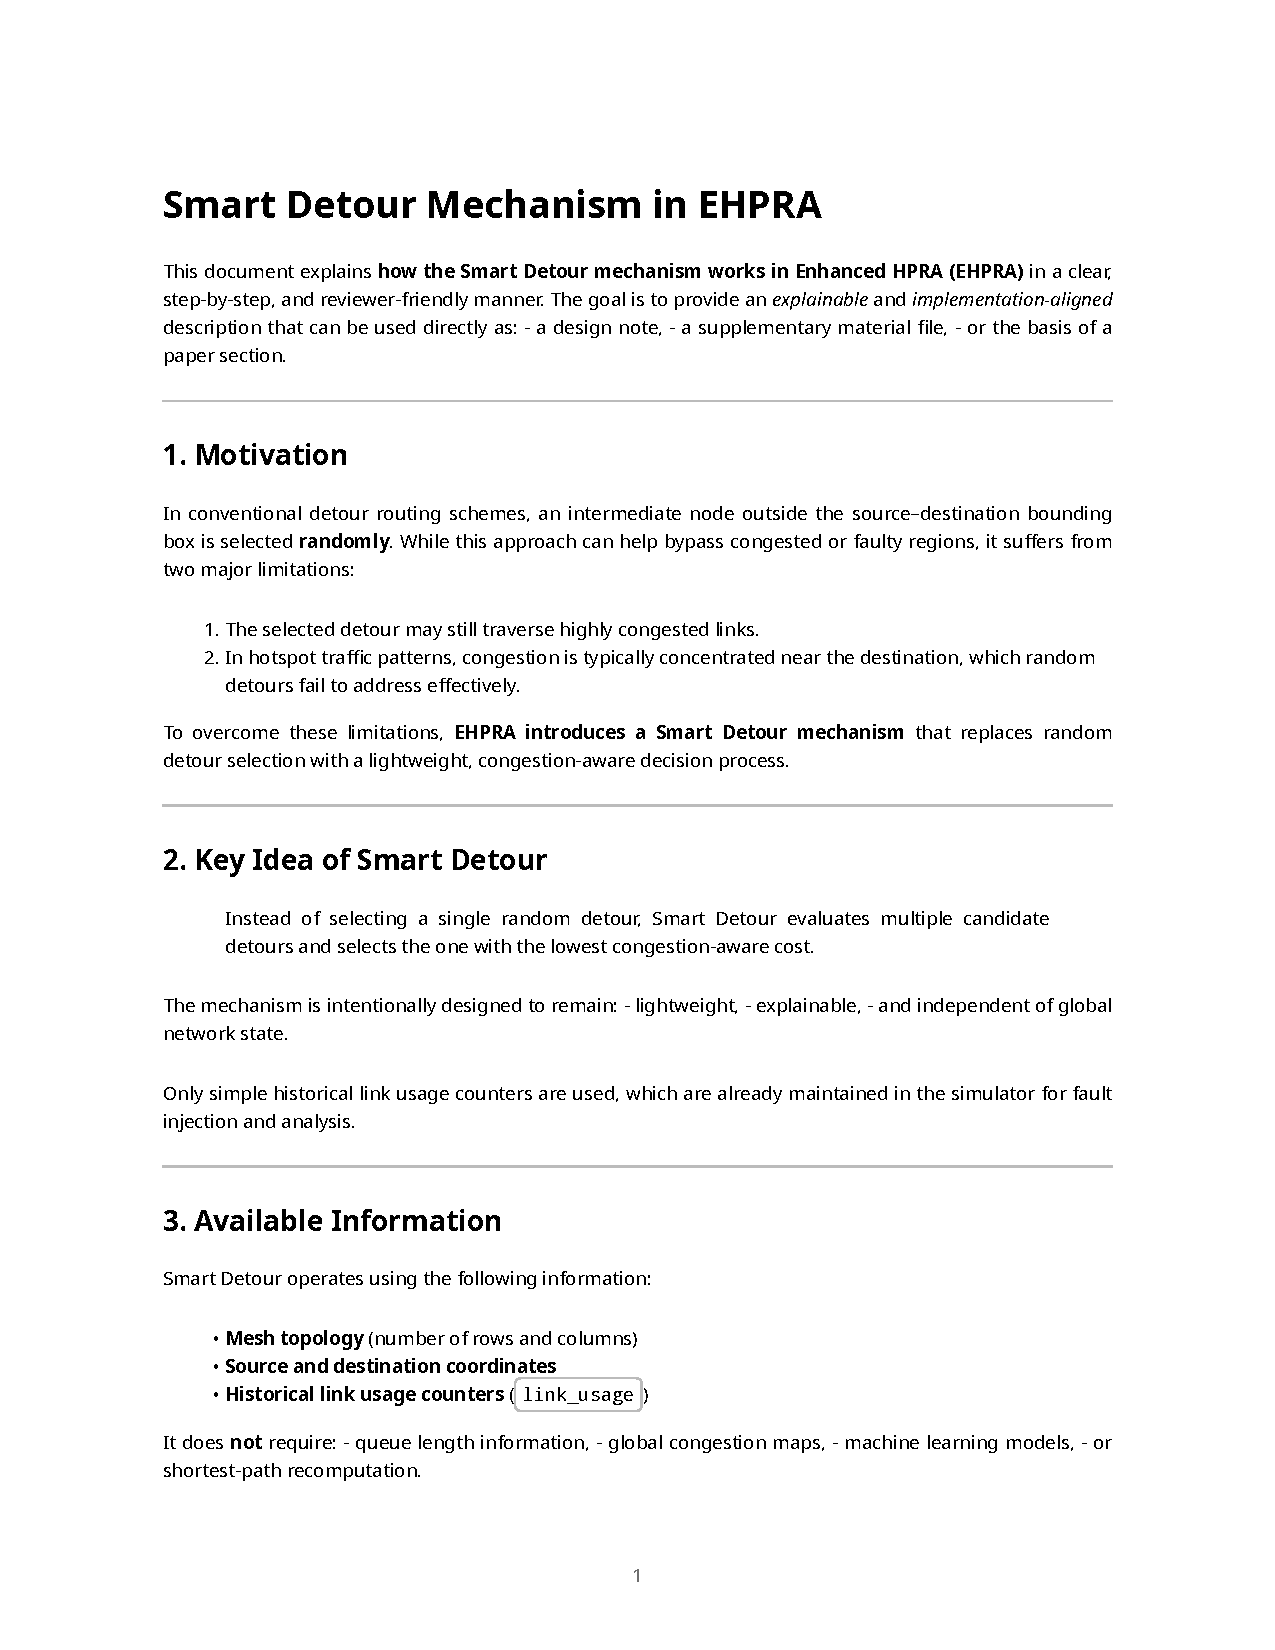
\includegraphics[page=1,width=0.9\textwidth]{Results/Smart Detour Explanation (ehpra).pdf}
    \caption{Smart Detour design concept used in EHPRA.}
\end{figure}

\section{Experimental Methodology}
\subsection{Implementation and Reproducibility}
Experiments are based on the project Python simulator with fixed random seeds for pseudo-random libraries. All algorithms are evaluated under identical topology, fault settings, and traffic generators. This ensures fair relative comparison.

\subsection{Topology and Workloads}
\begin{itemize}[leftmargin=6mm]
    \item Topology: 16$\times$16 mesh.
    \item Hotlink pair: source $(2,3)$, destination $(5,6)$.
    \item Hotspot destination: $(8,8)$ with random dynamic sources.
\end{itemize}

\subsection{Compared Algorithms}
\begin{enumerate}[leftmargin=6mm]
    \item EHPRA (proposed)
    \item HPRA
    \item Minimal-oblivious
    \item Random detour
    \item XY
\end{enumerate}

\subsection{Simulation Parameters}
Each algorithm is simulated for 1,000,000 trials per scenario. Fault period is 10 trials, fault duration is 5 trials, and hot-threshold for selecting candidate faulty links is 3. Adaptive parameters are $p_{up}=0.01$, $p_{down}=0.01$, and $p_{decay}=0.0005$.

\subsection{Reported Metrics}
\begin{itemize}[leftmargin=6mm]
    \item Total number of fault events.
    \item Average hops per trial.
    \item Weighted overall cost as in Eq. (1).
    \item Relative improvements of EHPRA over baselines.
\end{itemize}

\section{Results and Expanded Analysis}
\subsection{Hotspot Scenario}
\begin{table}[H]
\centering
\caption{Hotspot results (1,000,000 trials).}
\begin{tabular}{lcc}
\toprule
Algorithm & Total Faults & Avg Hops \\
\midrule
EHPRA & 150,320 & 13.02 \\
HPRA & 167,566 & 10.07 \\
Minimal & 193,770 & 10.03 \\
Detour & 232,711 & 25.43 \\
XY & 250,971 & 9.03 \\
\bottomrule
\end{tabular}
\end{table}

Compared with HPRA, EHPRA reduces faults by 10.29\%. Against Minimal and XY, the reduction is 22.42\% and 40.10\%, respectively. EHPRA pays additional hops relative to strict minimal methods, but this is expected in reliability-focused routing under destination-centric congestion.

\subsection{Hotlink Scenario}
\begin{table}[H]
\centering
\caption{Hotlink results (1,000,000 trials).}
\begin{tabular}{lcc}
\toprule
Algorithm & Total Faults & Avg Hops \\
\midrule
EHPRA & 213,375 & 12.66 \\
HPRA & 293,112 & 14.09 \\
Minimal & 375,388 & 8.00 \\
Detour & 458,702 & 28.83 \\
XY & 499,995 & 7.00 \\
\bottomrule
\end{tabular}
\end{table}

In hotlink traffic, EHPRA provides 27.20\% fewer faults than HPRA and 57.32\% fewer than XY. Importantly, EHPRA also improves hop count relative to HPRA (12.66 vs. 14.09), showing that informed detour candidate selection avoids long unnecessary detours.

\subsection{Weighted Cost Comparison}
Using $w_f=0.8$ and $w_h=0.2$:
\begin{itemize}[leftmargin=6mm]
    \item \textbf{Hotspot cost}: EHPRA $=0.5816$, HPRA $=0.6133$, Minimal $=0.6965$, Detour $=0.9418$, XY $=0.8710$.
    \item \textbf{Hotlink cost}: EHPRA $=0.4292$, HPRA $=0.5667$, Minimal $=0.6561$, Detour $=0.9339$, XY $=0.8486$.
\end{itemize}
EHPRA is the best algorithm by this reliability-prioritized metric in both scenarios.

\subsection{Reliability-Latency Trade-off Interpretation}
Results indicate that strict shortest-path behavior minimizes hops but repeatedly traverses vulnerable high-usage links. Smart detours intentionally increase path diversity and avoid recurrent fault-prone channels. The net effect is lower fault accumulation and better weighted system behavior for reliability-critical settings.

\subsection{Why Destination-Aware Weighting Helps}
Hotspot traffic naturally concentrates around sink-adjacent links. Penalizing congestion near destination increases the chance of entering the hotspot region from less-used directions. This relieves bottleneck pressure and reduces repeated selection of fragile destination-neighbor links.

\subsection{Ablation-Style Discussion}
Although full ablation experiments are future work, existing behavior supports three component-level effects:
\begin{enumerate}[leftmargin=6mm]
    \item HPRA-style adaptive $p$ adds dynamic exploration under faults.
    \item Smart candidate generation broadens detour alternatives.
    \item Destination-aware scoring ranks alternatives to avoid high-risk links.
\end{enumerate}
The combination produces the strongest observed reliability gains.

\begin{figure}[H]
    \centering
    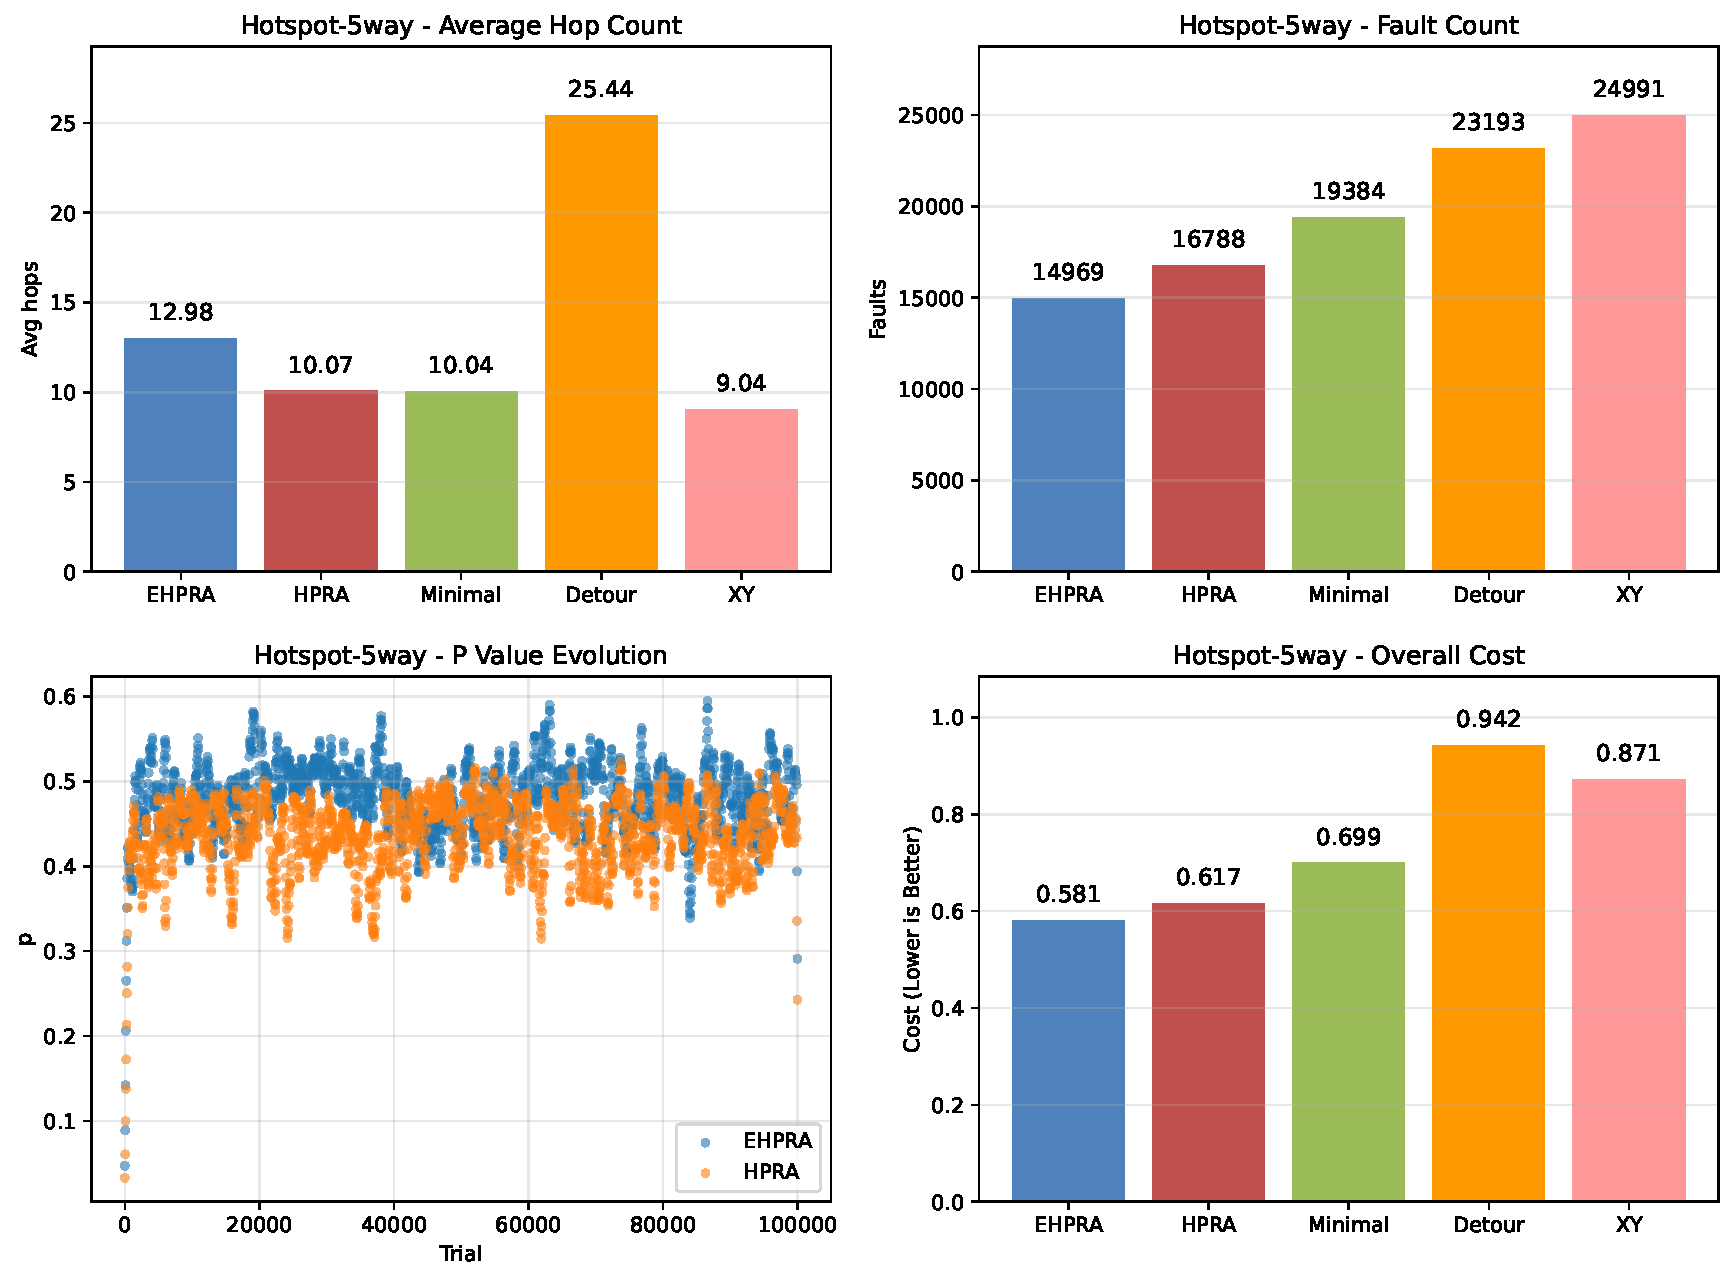
\includegraphics[width=0.92\textwidth]{Results/Hotspot-5way-figure.pdf}
    \caption{Five-way comparison in hotspot traffic (project-generated).}
\end{figure}

\begin{figure}[H]
    \centering
    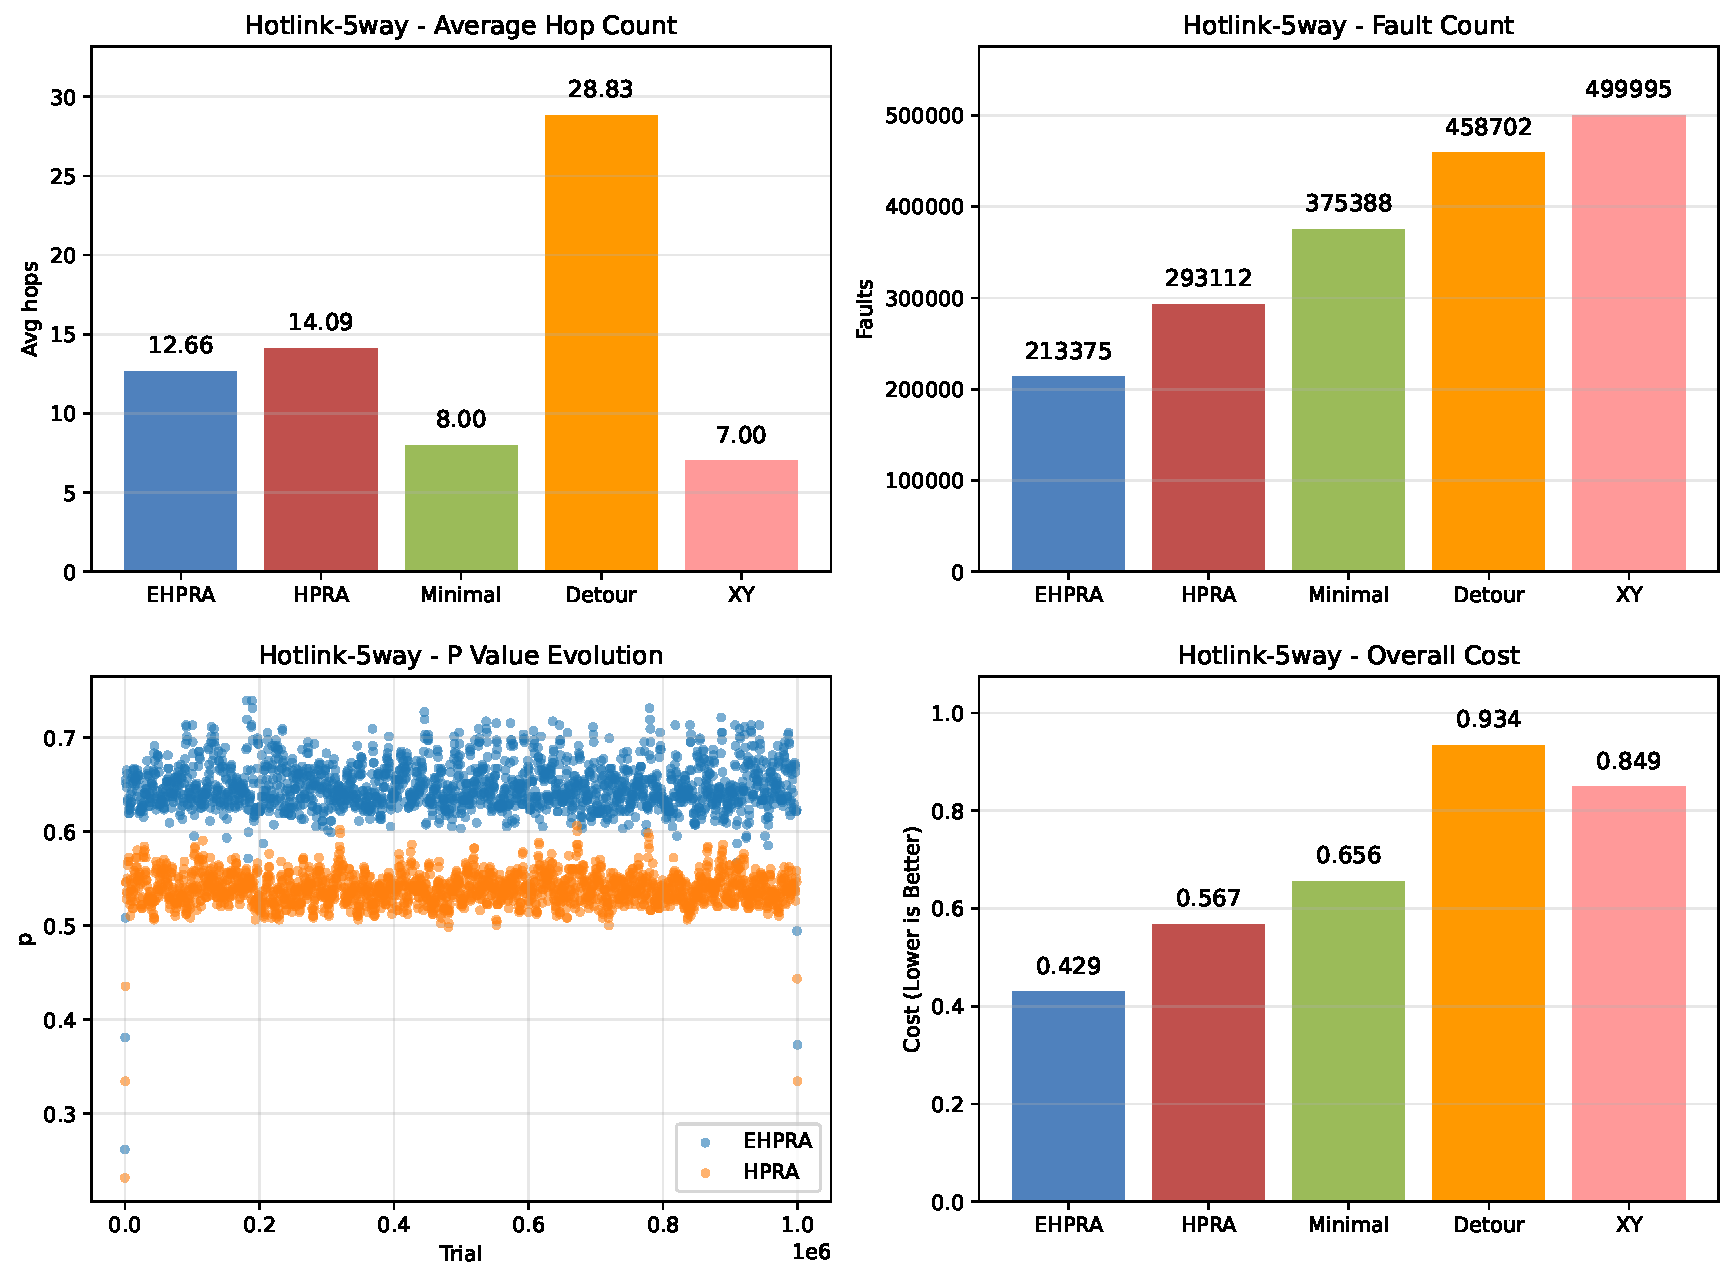
\includegraphics[width=0.92\textwidth]{Results/Hotlink-5way-figure.pdf}
    \caption{Five-way comparison in hotlink traffic (project-generated).}
\end{figure}

\section{Implementation Feasibility and Practical Considerations}
\subsection{Hardware-Oriented Suitability}
EHPRA avoids global traffic maps and learning-based inference. It uses bounded candidate evaluation, local link counters, and simple arithmetic operations, which are favorable for practical implementation compared with heavyweight optimization.

\subsection{Parameter Selection Guidance}
Three parameter groups influence behavior:
\begin{itemize}[leftmargin=6mm]
    \item Adaptation rates ($p_{up}, p_{down}, p_{decay}$): govern exploration dynamics.
    \item Candidate and hop terms ($k, \lambda$): govern detour quality and path inflation.
    \item Destination weighting factor (constant 6 in Eq. (4)): controls hotspot sensitivity.
\end{itemize}
In reliability-centric deployments, stronger fault penalty and moderate $\lambda$ are recommended.

\subsection{Threats to Validity}
This study is simulation-based and focuses on two canonical traffic patterns. While these are common stress tests, additional workloads (trace-driven, mixed QoS classes, bursty injection) and cycle-accurate hardware models should be explored in future work.


\section{Extended Quantitative Breakdown}
\subsection{Relative Improvement Tables}
To provide a clearer reviewer-facing summary, Tables~\ref{tab:hotspot_imp} and~\ref{tab:hotlink_imp} report relative fault reduction and hop-count variation of EHPRA against each baseline. Positive values in fault reduction are better. Hop variation is reported as percentage change of EHPRA relative to baseline, where negative means fewer hops and positive means more hops.

\begin{table}[H]
\centering
\caption{EHPRA relative improvements in hotspot traffic.}
\label{tab:hotspot_imp}
\begin{tabular}{lcc}
\toprule
Baseline & Fault Reduction (\%) & Hop Change (\%) \\
\midrule
HPRA & 10.29 & +29.29 \\
Minimal & 22.42 & +29.81 \\
Detour & 35.40 & -48.80 \\
XY & 40.10 & +44.19 \\
\bottomrule
\end{tabular}
\end{table}

\begin{table}[H]
\centering
\caption{EHPRA relative improvements in hotlink traffic.}
\label{tab:hotlink_imp}
\begin{tabular}{lcc}
\toprule
Baseline & Fault Reduction (\%) & Hop Change (\%) \\
\midrule
HPRA & 27.20 & -10.15 \\
Minimal & 43.16 & +58.25 \\
Detour & 53.48 & -56.09 \\
XY & 57.32 & +80.86 \\
\bottomrule
\end{tabular}
\end{table}

These tables clarify a practical point: EHPRA is not intended to always minimize hop count against strict-minimal baselines; instead, it minimizes a reliability-weighted objective. In reliability-focused systems, avoiding repeated faults often provides larger end-to-end performance benefit than preserving shortest-path hop count.

\subsection{Interpreting Cost Dominance}
Cost dominance of EHPRA is observed in both traffic modes. Let
\begin{equation}
\Delta C_{A\rightarrow E}=C_A-C_E
\end{equation}
where $C_E$ is EHPRA cost and $C_A$ is the cost of algorithm $A$. For hotspot traffic, the largest margin appears against Detour and XY, while for hotlink traffic EHPRA strongly dominates all baselines including HPRA. This consistent ordering indicates that Smart Detour improves routing quality under both destination-centric and corridor-centric pressure.

A key reason is that Smart Detour reduces repeated traversal probability on overused links while still constraining unnecessary path inflation through $\lambda\cdot H(P)$. Thus, EHPRA does not behave as unconstrained detour routing; it behaves as \emph{controlled exploration}.

\subsection{Expected Behavior Under Parameter Variation}
Although this work reports fixed canonical parameters, EHPRA behavior can be anticipated across tuning regimes:
\begin{itemize}[leftmargin=6mm]
    \item \textbf{Larger $p_{up}$}: faster transition to detour mode after faults, usually beneficial for bursty fault episodes but potentially noisier under short-lived disturbances.
    \item \textbf{Larger $p_{decay}$}: quicker return to minimal behavior, useful when faults are sparse and stability is preferred.
    \item \textbf{Larger $\lambda$}: stronger hop penalization, making EHPRA closer to minimal routing.
    \item \textbf{Larger candidate count $k$}: potentially better detour quality at higher per-packet evaluation cost.
\end{itemize}
The current parameter set is a balanced point between exploration quality and computational overhead.

\subsection{Scalability Considerations}
For larger meshes, destination-neighbor congestion typically becomes more critical in hotspot traffic. The distance-sensitive weight in Eq. (4) naturally addresses this by increasing relative penalty near the sink. However, candidate search should remain bounded for hardware feasibility. A practical approach is to keep $k$ fixed and adjust only $k_\Delta$ with mesh size.

In 3D mesh extensions, the same scoring framework can be retained by replacing Manhattan distance with 3D Manhattan distance and adding vertical-link usage counters. This indicates strong portability of the EHPRA design philosophy.

\subsection{Implications for NoC Design Space Exploration}
The presented results suggest that EHPRA is most attractive for design points where reliability carries higher value than strict latency minimization, including safety-aware accelerators, long-running embedded multicore platforms, and systems with expected thermal-induced link stress. The method can also complement DVFS and task-mapping strategies by reducing communication-side fragility.

From an architectural perspective, EHPRA demonstrates that meaningful routing gains are attainable without global state exchange or machine-learning inference. This keeps verification and integration complexity moderate and makes the method suitable for early-stage NoC design-space exploration.


\section{Conclusions and Future Work}
This paper presented EHPRA, an enhanced hybrid probabilistic routing method for 2D mesh NoC. By combining HPRA's adaptive mode-switching with Smart Detour candidate scoring, EHPRA significantly reduces fault exposure in both hotspot and hotlink conditions. Across one million trials per scenario, EHPRA consistently achieves the lowest fault count and best weighted overall cost among five compared algorithms.

The expanded analysis confirms that EHPRA improves reliability while maintaining acceptable path length, and in hotlink traffic it even outperforms HPRA in both metrics simultaneously. These findings make EHPRA a strong practical candidate for fault-aware NoC routing.

Future work includes parameter-space sweeps, cycle-accurate timing studies, extension to 3D mesh topologies, and QoS-aware or priority-aware Smart Detour variants.

\section*{Acknowledgments}
The authors acknowledge the support of the research environment and simulation framework developed at Amirkabir University of Technology for this study.

\section*{Nomenclature}
\begin{tabular}{>{\raggedright\arraybackslash}p{2.8cm}p{11cm}}
$p$ & Probability of selecting detour mode \\
$p_{up}$ & Increment in $p$ after fault in minimal mode \\
$p_{down}$ & Decrement in $p$ after fault in detour mode \\
$p_{decay}$ & Continuous decay term of $p$ \\
$U(u,v)$ & Historical usage of link $(u,v)$ \\
$\lambda$ & Hop-count penalty coefficient \\
$F$ & Total faults \\
$H$ & Average hops \\
$R, C$ & Mesh row and column counts \\
$\Delta$ & Detour radius factor derived from $p$ \\
\end{tabular}

\section*{References}
[1] A. Akhbari, H. Khoojooyan, and M. Tarighi, ``HPRA: Hybrid Probabilistic Routing Algorithm for 2D Mesh NoC,'' International Conference on Electrical, Computer and Mechanical Engineering.

[2] W. J. Dally and B. Towles, \emph{Principles and Practices of Interconnection Networks}. San Francisco, CA, USA: Morgan Kaufmann, 2004.

[3] L. Benini and G. De Micheli, ``Networks on chips: A new SoC paradigm,'' \emph{Computer}, vol. 35, no. 1, pp. 70--78, 2002.

[4] J. Duato, S. Yalamanchili, and L. Ni, \emph{Interconnection Networks: An Engineering Approach}. San Francisco, CA, USA: Morgan Kaufmann, 2002.

[5] P. P. Pande, C. Grecu, M. Jones, A. Ivanov, and R. Saleh, ``Performance evaluation and design trade-offs for network-on-chip interconnect architectures,'' \emph{IEEE Transactions on Computers}, vol. 54, no. 8, pp. 1025--1040, 2005.

[6] E. J. Kim, K. H. Yum, G. M. Link, N. Vijaykrishnan, M. Kandemir, M. J. Irwin, M. Yousif, and C. R. Das, ``Adaptive network routing for irregular applications in chip multiprocessors,'' \emph{Proceedings of DAC}, pp. 130--135, 2005.

[7] T. Bjerregaard and S. Mahadevan, ``A survey of research and practices of Network-on-chip,'' \emph{ACM Computing Surveys}, vol. 38, no. 1, Article 1, 2006.

[8] J. Hu and R. Marculescu, ``DyAD: Smart routing for networks-on-chip,'' \emph{Proceedings of DAC}, pp. 260--263, 2004.

\end{document}
